\begin{landscape}
\begin{figure}
    \centering

	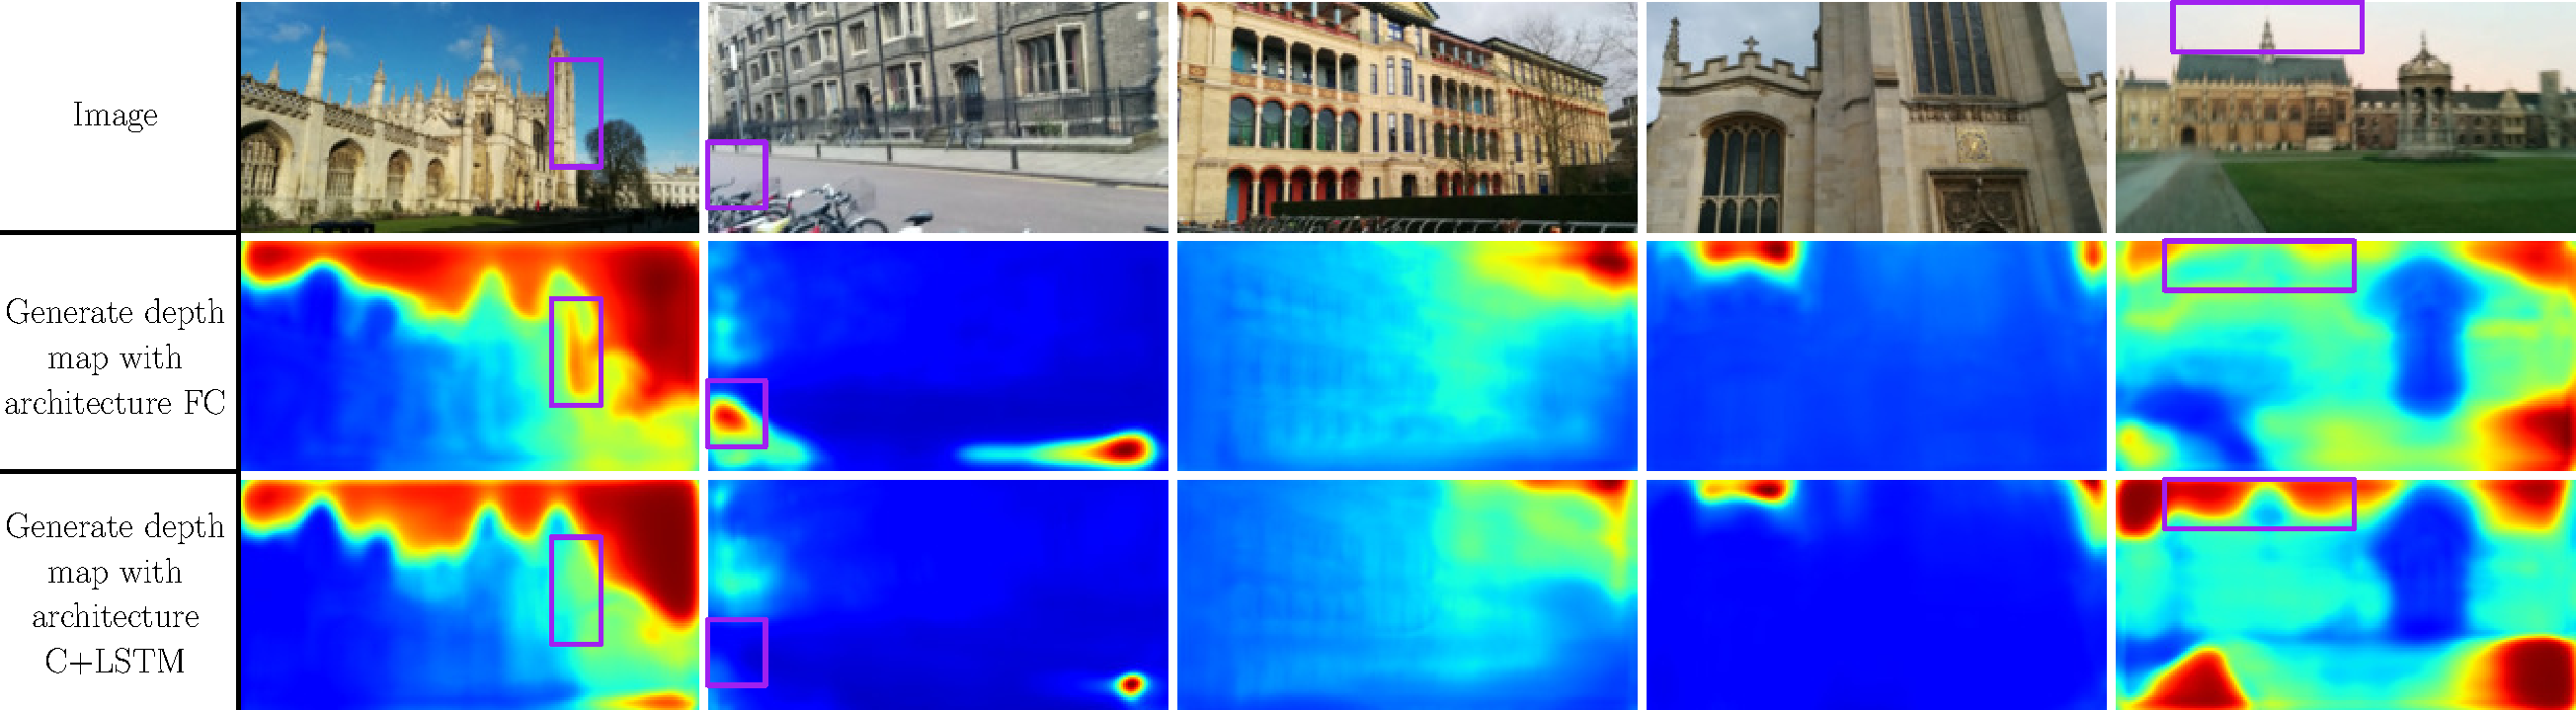
\includegraphics[width=\linewidth]{results/outdoor/depth_maps}
	\caption[Generated outdoor depth maps]{\label{fig:depth_map_outdoor} Visualisation of the depth map generated from RGB input by our two architectures, FC and C+LSTM, trained in an unsupervised manner on Cambridge Landmarks dataset~\citep{Kendall2015}. \textcolor{purple}{Purple boxes} show regions where C+LSTM network produces slightly better depth map reconstruction compared to FC.}
	
\end{figure}
\end{landscape}